%------------------------------------------------------------------------------------------------------------
%	PACKAGES AND DOCUMENT CONFIGURATIONS
%------------------------------------------------------------------------------------------------------------

\documentclass[12pt]{article} % Document Type and font dimension
\usepackage[utf8]{inputenc} % Import package to read letters with accents
\usepackage[T1]{fontenc} % Import package for font coding
\usepackage[italian]{babel} % Language of the document
\usepackage{inconsolata} % Font of the document
\usepackage[a4paper, margin=1.3in]{geometry} % Set margin
\usepackage{multicol}
\usepackage{graphicx} % Import packages for images
\usepackage[export]{adjustbox}
%\usepackage{minted} % Import package to render vhdl code
\usepackage{tocloft} % Import to add dots to the table of contents
\usepackage{scrlayer} % Import packages for layers - front page
\usepackage{scrhack} 
\usepackage{sidecap} % Import packages for captions
\usepackage{hyperref} % Import for hyperrefs
\usepackage{tabularborder}
\usepackage{multirow} % multi rows
\usepackage{multicol} % multi colums
\usepackage{amsmath}
\usepackage{pdfpages} % Import for importing pdfs
\usepackage{float}

\renewcommand{\cftsecdotsep}{2} % table of content setup
\renewcommand{\cftsubsecdotsep}{2}
\renewcommand*{\thefootnote}{(\arabic{footnote})} % footnote setup

\hypersetup{ % hyperlinks color setup
	colorlinks,
	citecolor=black,
	filecolor=black,
	linkcolor=black,
	urlcolor=black
}

\DeclareNewLayer[ % Footnote setup
	background,
	textarea,
	addwidth=\footskip,
	addwidth=\footheight,
	contents=\hfill
	\rotatebox{90}{\parbox{\layerheight}{\centering\pagemark}}]{lscape.foot}
\DeclareNewPageStyleByLayers{lscape}{lscape.foot}

\graphicspath{{images/}} % define path for images

%------------------------------------------------------------------------------------------------------------
%	TITLE PAGE
%------------------------------------------------------------------------------------------------------------

\begin{document}
	\begin{titlepage}
		%
		\centering
		%
		\includegraphics[width=100pt]{Logo_Politecnico_Milano}\par
		%
		\vspace{1cm}
		%
		{\scshape\Large Progetto Finale di Reti Logiche \par}
		%
		\vspace{1.5cm}
		%
		{\huge\bfseries Codificatore Convoluzionale\par}
		%
		\vspace{2cm}
		%
		%{\Large \textit{Giovanni Manfredi}\par}
		\begin{multicols}{2}
			%
			\begin{tabular}{l r}
				Giovanni Manfredi\\
				Matricola: & 937160\\ 
				Codice Persona: & 10708042
			\end{tabular}
			%
			\begin{tabular}{l r}
				Sebastiano Meneghin\\
				Matricola: & 937058\\ 
				Codice Persona: & 10627650
			\end{tabular}
			%
		\end{multicols}
		\vspace{6.5cm}
		supervisore\par
		Prof.\ Fabio \textsc{Salice}
		\vfill
		{\large 15 giugno 2022 \par}
		%
	\end{titlepage}
	%
	\tableofcontents
	\newpage
	%
%------------------------------------------------------------------------------------------------------------
%	SECTION 1 - INTRODUCTION
%------------------------------------------------------------------------------------------------------------
	%
	\section{Introduzione}
	\label{sec:Introduzione}
		%
		\subsection{Analisi delle specifiche}
			%
			Lo scopo del progetto è l'implementazione di un componente hardware, 
			descritto in VHDL, che interfacciandosi con la memoria esegua l'operazione seguente. 
			
			L'elemento implementato va a \textbf{leggere} parole da otto bit (o un byte) 
			da una memoria RAM, per poi andarle a \textbf{serializzare} in un flusso continuo di un bit, 
			che arriva in input ad un \textbf{convolutore} (secondo lo schema riportato 
			in Figura \ref{fig:ConvolutoreDataPath}). Questo codifica il suo ingresso in  
			un flusso in uscita di due bit, che vengono conseguentemente 
			\textbf{deserializzati} e \textbf{scritti} in memoria.
			%
			\begin{figure}[h]
				\centering
				\includegraphics[width=12cm]{ConvolutoreDataPath.jpg}
				\caption{Data path del convolutore}
				\label{fig:ConvolutoreDataPath}
			\end{figure}
			%
			\begin{figure}[h]
				\centering
				\includegraphics[width=\textwidth]{ConvolutoreFSM.jpg}
				\caption{Finite State Machine (FSM) del convolutore}
				\label{fig:ConvolutoreFSM}
			\end{figure}
			%
		\subsection{Esempio}
			%
			Vediamo ora alcuni esempi riguardanti il funzionamento del componente hardware, 
			mostrando i numeri letti e scritti in memoria
			
			\begin{align*}
				W &: 1010 \ 1100 \quad 0101 \ 1111 \\
				Z &:  1101 \ 0001 \ 0010 \ 1011 \quad 0011 \ 0100 \ 1001 \ 0101
			\end{align*}
			\begin{table}[h!]
				\centering
				\begin{tabular}{ccr}
					\toprule
					INDIRIZZO MEMORIA & VALORE & COMMENTO \\
					\midrule
					0 & 2 & Byte lunghezza sequenza di ingresso \\
					\midrule
					1 & 172 & Primo byte in sequenza da codificare \\
					\midrule
					1 & 95 &  \\
					\midrule
					... &   0 & Memoria vuota \\
					\midrule
					1000 & 209 & Primo byte sequenza di uscita \\
					\midrule
					1001 & 43 & \\
					\midrule
					1002 &  52 & \\
					\midrule
					1003 & 149 & \\			
					\bottomrule
				\end{tabular}
				\caption{Esempio 1 - Sequenza di lunghezza 2}
				\label{tab:1}
			\end{table}
			\newpage
			\begin{align*}
				W : \ &1000 \ 0011 \quad 0000 \ 1100 \\ 
					   &0101 \ 1101 \quad 0010 \ 1001 \\ 
					   &0011 \ 1111 \quad 0000 \ 0110 \\
				Z :  \ &1101 \ 1100 \ 0000 \ 1110  \quad 1011 \ 0000 \ 1110 \ 1011 \\
				     &0011 \ 0100 \ 1001 \ 1000 \quad 0111 \ 1101 \ 0001 \ 1111 \\
				     &0111 \ 1110 \ 0101 \ 0101 \quad  1011 \ 0000 \ 0011 \ 1010 
			\end{align*}
			\begin{table}[h!]
				\centering
				\begin{tabular}{ccr}
					\toprule
					INDIRIZZO MEMORIA & VALORE & COMMENTO \\
					\midrule
					0 & 6 & Byte lunghezza sequenza di ingresso \\
					\midrule
					1 & 131 & Primo byte in sequenza da codificare \\
					\midrule
					1 & 12 &  \\
					\midrule
					1 & 93 &  \\
					\midrule
					1 & 41 &  \\
					\midrule
					1 & 63 &  \\
					\midrule
					1 & 6 &  \\
					\midrule
					... &   0 & Memoria vuota \\
					\midrule
					1000 & 209 & Primo byte sequenza di uscita \\
					\midrule
					1001 & 14 & \\
					\midrule
					1002 &  176 & \\
					\midrule
					1003 &  235 & \\
					\midrule
					1004 & 52 & \\
					\midrule
					1005 & 152 &  \\
					\midrule
					1006 & 125 &  \\
					\midrule
					1007 & 31 &  \\
					\midrule
					1008 & 126 &  \\
					\midrule
					1009 & 85 &  \\
					\midrule
					1010 & 176 &  \\
					\midrule
					1011 & 58 &  \\
					\bottomrule
				\end{tabular}
				\caption{Esempio 2 - Sequenza di lunghezza 6}
				\label{tab:2}
			\end{table}
			\newpage
			%
		\subsection{Approccio progettuale}
			%
			Ci siamo approcciati al progetto andando ad individuare quali fossero i singoli passaggi 
			che il componente esegue per realizzare l'operazione richiesta. 
			Abbiamo individuato cinque \textit{\textbf{steps}} principali:
			%
			\begin{itemize}
				\item \textbf{Lettura da memoria}
				\item \textbf{Trasformazione parallela - seriale}
				\item \textbf{Convolutore}
				\item \textbf{Trasformazione seriale - parallela}
			\end{itemize}
			%
			Abbiamo inoltre notato la necessità di tenere d'occhio altri due elementi 
			che se non gestiti bene potrebbero essere problematici: \textbf{il ciclo di clock} e i \textbf{buffer}. 
			
			Data la natura \textbf{sincrona} del processo, 
			nella lettura da memoria dovremo "aspettare il valore" 
			un ciclo di clock in più (rispetto ad un processo asincrono). 
			Per quanto riguarda \textbf{il tempo di clock}, visto il funzionamento del convolutore 
			(ricava due bit da uno) "\textit{il tempo}" sarà scandito dalla parte di scrittura in memoria,
			in quanto non potremo leggere una nuova parola finché non avremo salvato entrambe 
			le parole in output al convolutore.
			\newline
			
			Siamo quindi andati a delinare un \textbf{Data path} che descrivesse il circuito
			del componente che abbiamo poi controllato tramite dei segnali di una 
			\textbf{Macchina a Stati Finiti o Finite State Machine - FSM}. 
			Le immagini e le descrizioni dettagliate del circuito e macchina a stati %della
			sono nella Sezione \ref{sec:Architettura}.
			
			\newpage
			%
%------------------------------------------------------------------------------------------------------------
%	SECTION 2 - ARCHITECTURE
%------------------------------------------------------------------------------------------------------------
	%
	\section{Architettura}
	\label{sec:Architettura}
		Come introdotto nell'introduzione (Sezione \ref{sec:Introduzione}) andremo a vedere
		lo schema del \textbf{Data path} e a spiegarne nel dettaglio i suoi punti e la \textbf{FSM}
		che lo controlla.
		%
		\subsection{Data path}
		\label{sec:Data_path}
			Qui sotto riportato in Figura \ref{fig:Data_path} l'intero Data path che andremo ad 
			analizzare più nel dettaglio in questo capitolo. 
			Specificati in figura ci sono anche i segnali di controllo gestiti dalla FSM e 
			per ogni flusso è specificato il numero di bit.
			\begin{figure}[h]
				\centering
				\includegraphics[width=\textwidth]{Data_path.jpg}
				\caption{Data path}
				\label{fig:Data_path}
			\end{figure}
			\newpage
			%		
			\subsubsection{Lettura da memoria e serializzazione}
				La prima sezione è dedicata alla \textbf{lettura da memoria} e \textbf{serializzazione}. 
				La lettura dalla memoria avviene in parole da 8 bit, che il processo salva  
				sul registro $reg_1$. Da questo registro, servendosi di un \textbf{multiplexer}, 
				genera un flusso  da 1 bit ($ u_k$) (serializzazione).
				\begin{figure}[h]
					\centering
					\includegraphics[width=0.5\textwidth]{Data_path_letturaMemoria.jpg}
					\caption{Lettura da memoria e serializzazione}
					\label{fig:Data_path_letturaMemoria}
				\end{figure}
			%
			\subsubsection{Convolutore}
				Dal flusso $ u_k$, seguendo lo schema indicato dalla specifica, si arriva al \textbf{convolutore}, 
				che svolge l'operazione salvando il risultato (di 2 bit) nel registro $reg_2$. Si notino i vari
				selettori utilizzati per resettare lo stato del convolutore.
				\begin{figure}[h]
					\centering
					\includegraphics[width=\textwidth]{Data_path_convolutore.jpg}
					\caption{Convolutore operazionale}
					\label{fig:Data_path_convolutore}
				\end{figure}
			%
			\subsubsection{Deserializzazione e Scrittura in memoria}
				Dal registro $reg_2$ si genera un flusso di 2 bit che utilizzando un \textbf{decoder} 
				(che deserializza il flusso) viene salvato nel registro $reg_3$ da 8 bit, 
				che verrà poi \textbf{scritto in memoria}.
				\begin{figure}[h]
					\centering
					\includegraphics[width=0.7\textwidth]{Data_path_scritturaMemoria.jpg}
					\caption{Deserializzazione e scrittura in memoria}
					\label{fig:Data_path_scritturaMemoria}
				\end{figure}
			%
			\subsubsection{Contatore}
				Parallelamente all'operazione principale (ovvero: lettura $\rightarrow$ serializzazione
				$\rightarrow$ convolutore $\rightarrow$ deserializzazione $\rightarrow$ scrittura)
				il processo \textbf{conta} il numero di volte che traduce una parola. 
				Visto che nel primo indirizzo (l'indirizzo 0) è presente il numero di parole da leggere, 
				una volta che il contatore sarà arrivato a zero il componente imposterà
				il \textbf{segnale di} $o_{end} = 1$ . 
				Si noti che bisogna prestare particolare attenzione nella FSM 
				a quando decrementare il contatore.
				\begin{figure}[h]
					\centering
					\includegraphics[width=0.7\textwidth]{Data_path_contatore.jpg}
					\caption{Contatore}
					\label{fig:Data_path_contatore}
				\end{figure}
			%
			\subsubsection{Indirizzo di lettura}
				Per aggiornare correttamente l'indirizzo di lettura da memoria si è pensato all'uso di un modulo
				a sé stante. L'indirizzo di lettura da memoria  è \textbf{inizializzato a 0}  nel registro $add_{in}$ 
				e aumentato di 1 ogni volta che il processo deve leggere una nuova parola.
				\begin{figure}[h]
					\centering
					\includegraphics[width=0.7\textwidth]{Data_path_indirizzoLettura.jpg}
					\caption{Indirizzo di lettura}
					\label{fig:Data_path_indirizzoLettura}
				\end{figure}
			%
			\subsubsection{Indirizzo di scrittura}
				Per aggiornare correttamente l'indirizzo di scrittura in memoria si è pensato all'uso di un modulo
				a sé stante. L'indirizzo di scrittura in memoria è \textbf{inizializzato a 1000}  nel registro $add_{out}$ 
				e aumentato di 1 ogni volta che il processo deve scrivere una nuova parola.
				\begin{figure}[h]
					\centering
					\includegraphics[width=0.7\textwidth]{Data_path_indirizzoScrittura.jpg}
					\caption{Indirizzo di scrittura}
					\label{fig:Data_path_indirizzoScrittura}
				\end{figure}
			%
		\subsection{Finite State Machine - FSM}
			La macchina a stati (FSM) controlla il Data path visto nella sezione \ref{sec:Data_path}. 
			Vedremo ora come funziona la sequenza di esecuzione del programma  e quali sono le sezioni che lo 
			compongono. Si noti che in tutti i cambi di stato (indicati con le frecce) avvengono sul fronte
			di salita del clock ($i_{ck}$).
			\begin{figure}[h]
				\centering
				\includegraphics[width=\textwidth]{FSM.jpg}
				\caption{FSM}
				\label{fig:FSM}
			\end{figure}
			%
			\subsubsection{Stato di reset e inizializzazione}	
				Il processo non inizia finché non riceve il segnale di $i_{start} = 1$. Dopo averlo ricevuto avviene la
				lettura del primo numero in memoria (all'indirizzo 0) che indica il \textbf{numero di parole} da tradurre.
				Questo numero iniziale viene caricato nel registro $reg_4$ e quindi in $reg_5$. Questa sezione 
				finisce con il controllo lato contatore: se questo è 0 la traduzione termina, andando 
				allo stato $S27$, altrimenti prosegue nello stato $S5$.
				\begin{figure}[h]
					\centering
					\includegraphics[width=0.5\textwidth]{FSM_inizializzazione.jpg}
					\caption{Stato di reset e inizializzazione}
					\label{fig:FSM_inizializzazione}
				\end{figure}
				\newpage
			%
			\subsubsection{Lettura e scrittura prima parola (byte)}
			\label{sec:LetturaScrittura_primaParola}
				Avendo verificato che il primo numero salvato in memoria (il numero di parole) sia diverso da zero,
				il processo esegue la fase di lettura, convoluzione e scrittura per almeno una parola.
				
				La lettura del primo byte è diversa dalla iterazioni successive alla prima, in quanto si deve
			    re-inizializzare il convolutore prima di usarlo. Come detto precedentemente, vista la natura
			    \textbf{sincrona} della memoria, è necessario aspettare due stati per poter avere
			    a disposizione il dato dalla memoria.
			    Alla fine della scrittura di entrambe le parole in memoria 
			    (da ciascuna parola in memoria ne vengono generate due), viene decrementato il contatore 
			    e verificato se è stato azzerato.
				\begin{figure}[h]
					\centering
					\includegraphics[width=0.9\textwidth]{FSM_letturabyte1.jpg}
					\caption{Lettura e scrittura della prima parola da memoria}
					\label{fig:FSM_letturabyte1}
				\end{figure}
			%
			\subsubsection{Lettura e scrittura parole successive alla prima}
				Se il contatore di parole non si è azzerato, l'operazione continua, andando a leggere una 
				nuova parola da memoria, seguendo lo stesso procedimento di prima, ma senza 
				la preoccupazione di resettare il convolutore. Anche alla fine di questa sezione 
				verifichiamo, decrementando il contatore, se esso è stato portato
				a 0. Si noti che viene riutilizzata la seconda parte della lettura e 
				scrittura della Sezione \ref{sec:LetturaScrittura_primaParola}.
				\begin{figure}[h]
					\centering
					\includegraphics[width=0.8\textwidth]{FSM_letturabyte2.jpg}
					\caption{Lettura e scrittura delle parole successive alla prima da memoria}
					\label{fig:FSM_letturabyte2}
				\end{figure}
				\newpage
			%
			\subsubsection{Terminazione}
				Una volta che dallo stato $S4$ oppure $S19$ viene sollevato il segnale $o_{end}$
				il processo va nello stato $S27$. Da questo stato
				il componente imposta il segnale $o_{done} = 1$ e attende che $i_{start}$ sia abbassato 
				per resettare $o_{done} = 0$ e quindi tornare allo stato di RESET ($S0$). 
				\begin{figure}[h]
					\centering
					\includegraphics[width=\textwidth]{FSM_terminazione.jpg}
					\caption{Terminazione}
					\label{fig:FSM_terminazione}
				\end{figure}
				\newpage
	%		
%------------------------------------------------------------------------------------------------------------
%	SECTION 3 - EXPERIMENTAL RESULTS
%------------------------------------------------------------------------------------------------------------
	%
	\section{Risultati Sperimentali}
		%
		\subsection{Sintesi}
			Il progetto è stato realizzato e testato sulla versione di \textbf{Vivado 2018.3}, utilizzando come
			FPGA target \textbf{xc7a200tfbg484-1}, e ha generato il seguente report di sintesi:\\
			
			\begin{tabular}{lcccc}
				\toprule
				Site Type                   & Used & Fixed & Available & Util\% \\
				\midrule
				Slice LUTs*                 & 94   & 0     & 134600    & 0.07   \\
				\quad LUT as Logic          & 94   & 0     & 134600    & 0.07   \\
				\quad LUT as Memory         & 0    & 0     & 46200     & 0.00   \\
				Slice Registers             & 73   & 0     & 269200    & 0.03  \\
				\quad Register as Flip Flop & 73    & 0     & 269200    & 0.03  \\
				\quad Register as Latch     & 0   & 0     & 269200    & 0.00  \\
				F7 Muxes                    & 1    & 0     & 67300     & <0.01   \\
				F8 Muxes                    & 0    & 0     & 33650     & 0.00   \\
				\bottomrule
		\end{tabular} \\ \\ \\
		
		Per il consumo invece: 
		
		\begin{figure}[H]
			\centering
			\includegraphics[width=\textwidth]{Report_Power.jpg}
			\caption{Consumi e potenza}
			\label{fig:Report_Power}
		\end{figure}
		\newpage
		\subsection{Schematics}
			In seguito una serie di immagini che mostrano come i circuiti sono stati descritti internamente
			da Vivado.
			\begin{figure}[H]
				\centering
				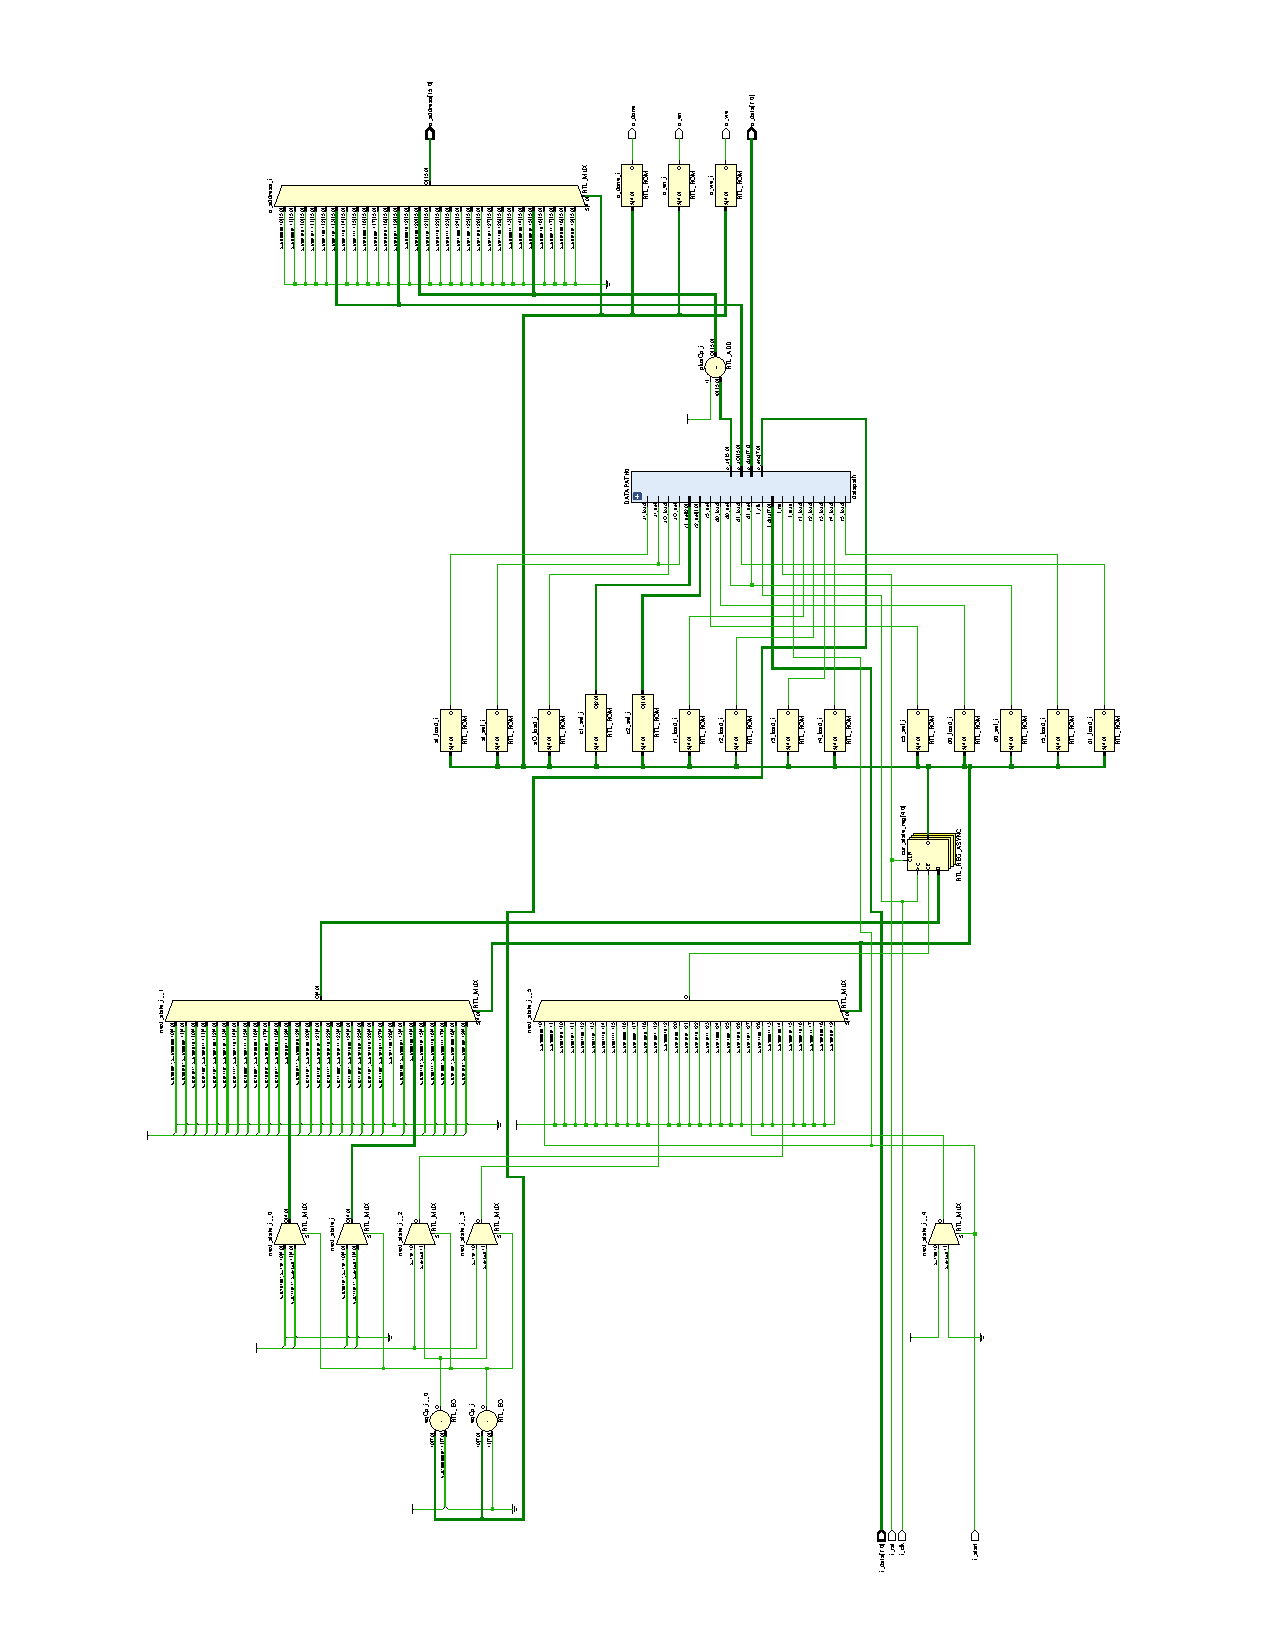
\includegraphics[width=\textwidth]{RTL_Closed_Schematic.pdf}
				\caption{Circuto in pre-sintesi con datapath non esplicito}
				\label{fig:Schematic_RTL_Closed}
			\end{figure}
			\begin{figure}[H]
				\centering
				\includegraphics[width=1.1\textwidth]{RTL_DataPath_Schematic.pdf}
				\caption{Circuto in pre-sintesi del datapath}
				\label{fig:Schematic_RTL_DataPath}
			\end{figure}
			\begin{figure}[H]
				\centering
				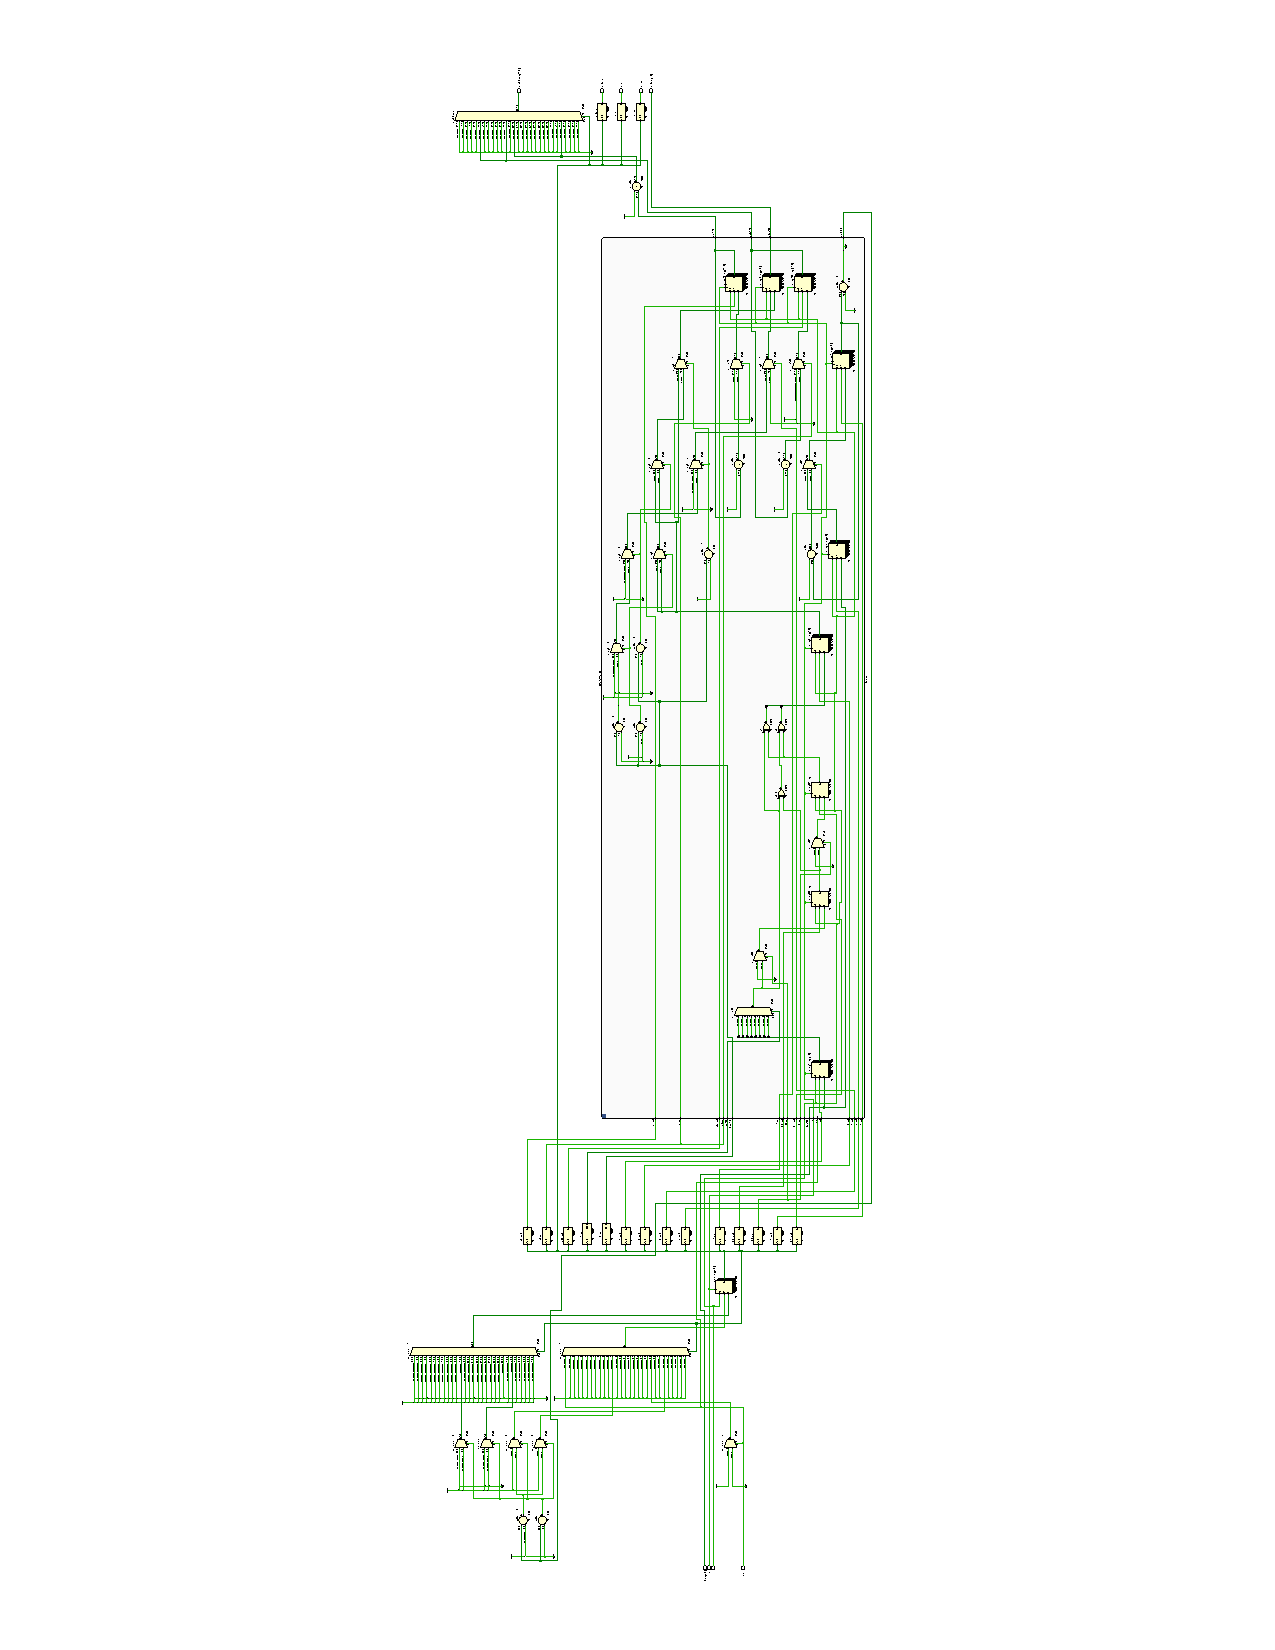
\includegraphics[width=1.1\textwidth]{RTL_Opened_Schematic.pdf}
				\caption{Circuto in pre-sintesi completo}
				\label{fig:Schematic_RTL_Opened}
			\end{figure}
			\begin{figure}[H]
				\centering
				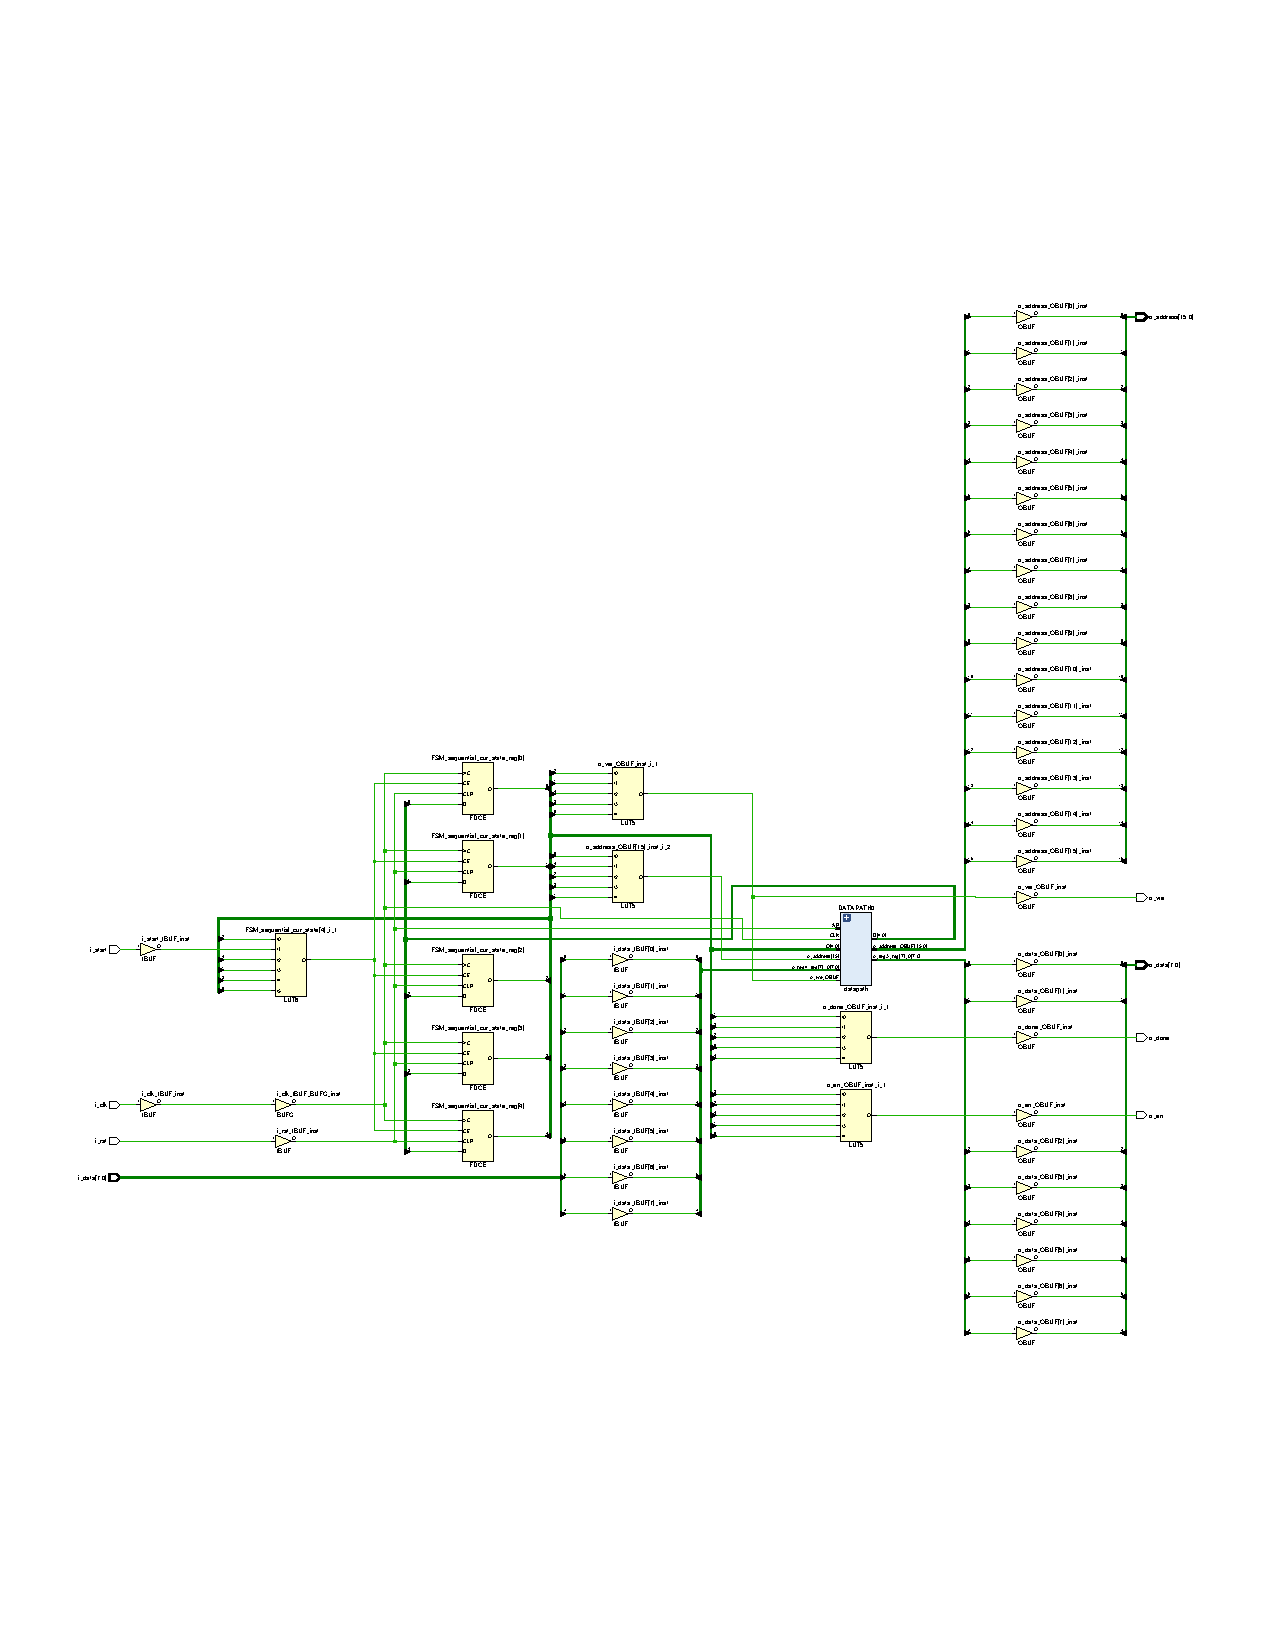
\includegraphics[width=1.1\textwidth]{PostSynthesis_Closed_Schematic.pdf}
				\caption{Circuto in post-sintesi con datapath non esplicito}
				\label{fig:Schematic_PostSynthesis_Closed}
			\end{figure}
			\begin{figure}[H]
				\centering
				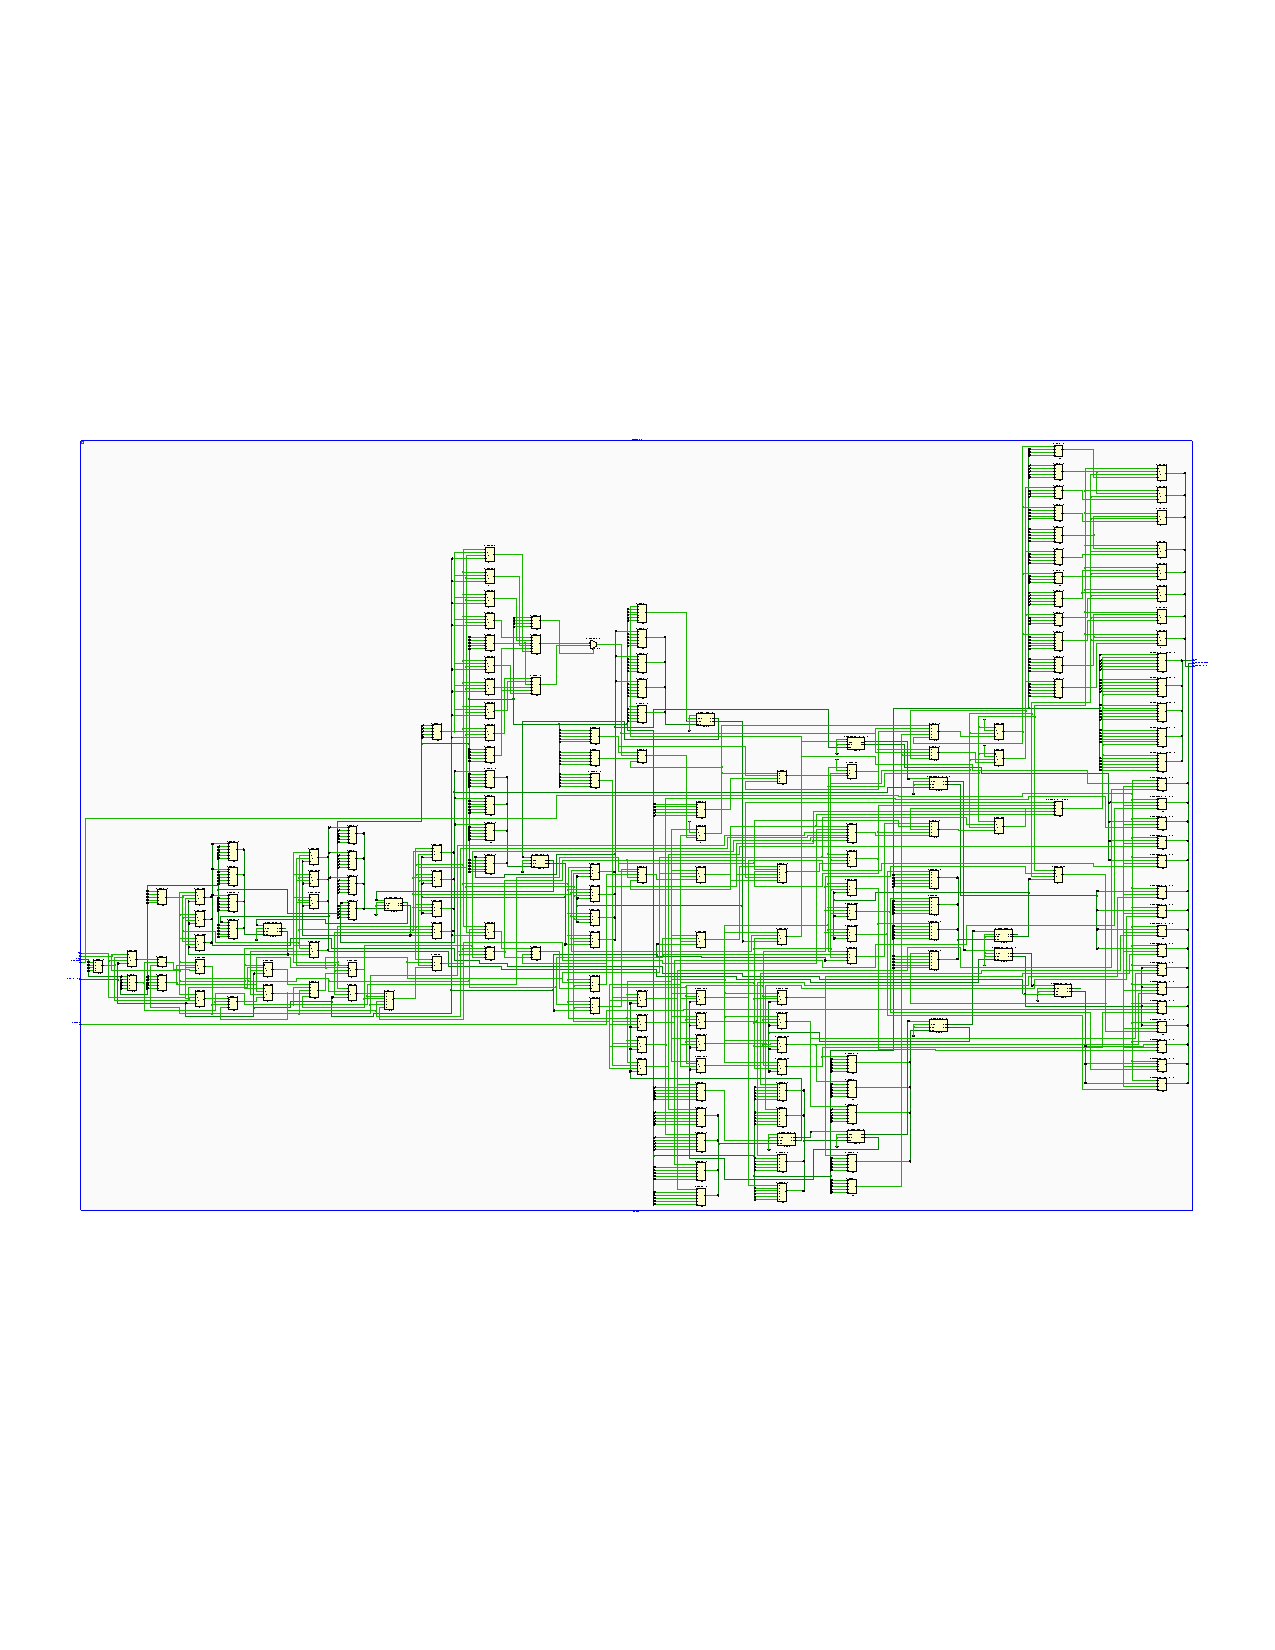
\includegraphics[width=1.1\textwidth]{PostSynthesis_DataPath_Schematic.pdf}
				\caption{Circuto in post-sintesi del datapath}
				\label{fig:Schematic_PostSynthesis_DataPath}
			\end{figure}
			\begin{figure}[H]
				\centering
				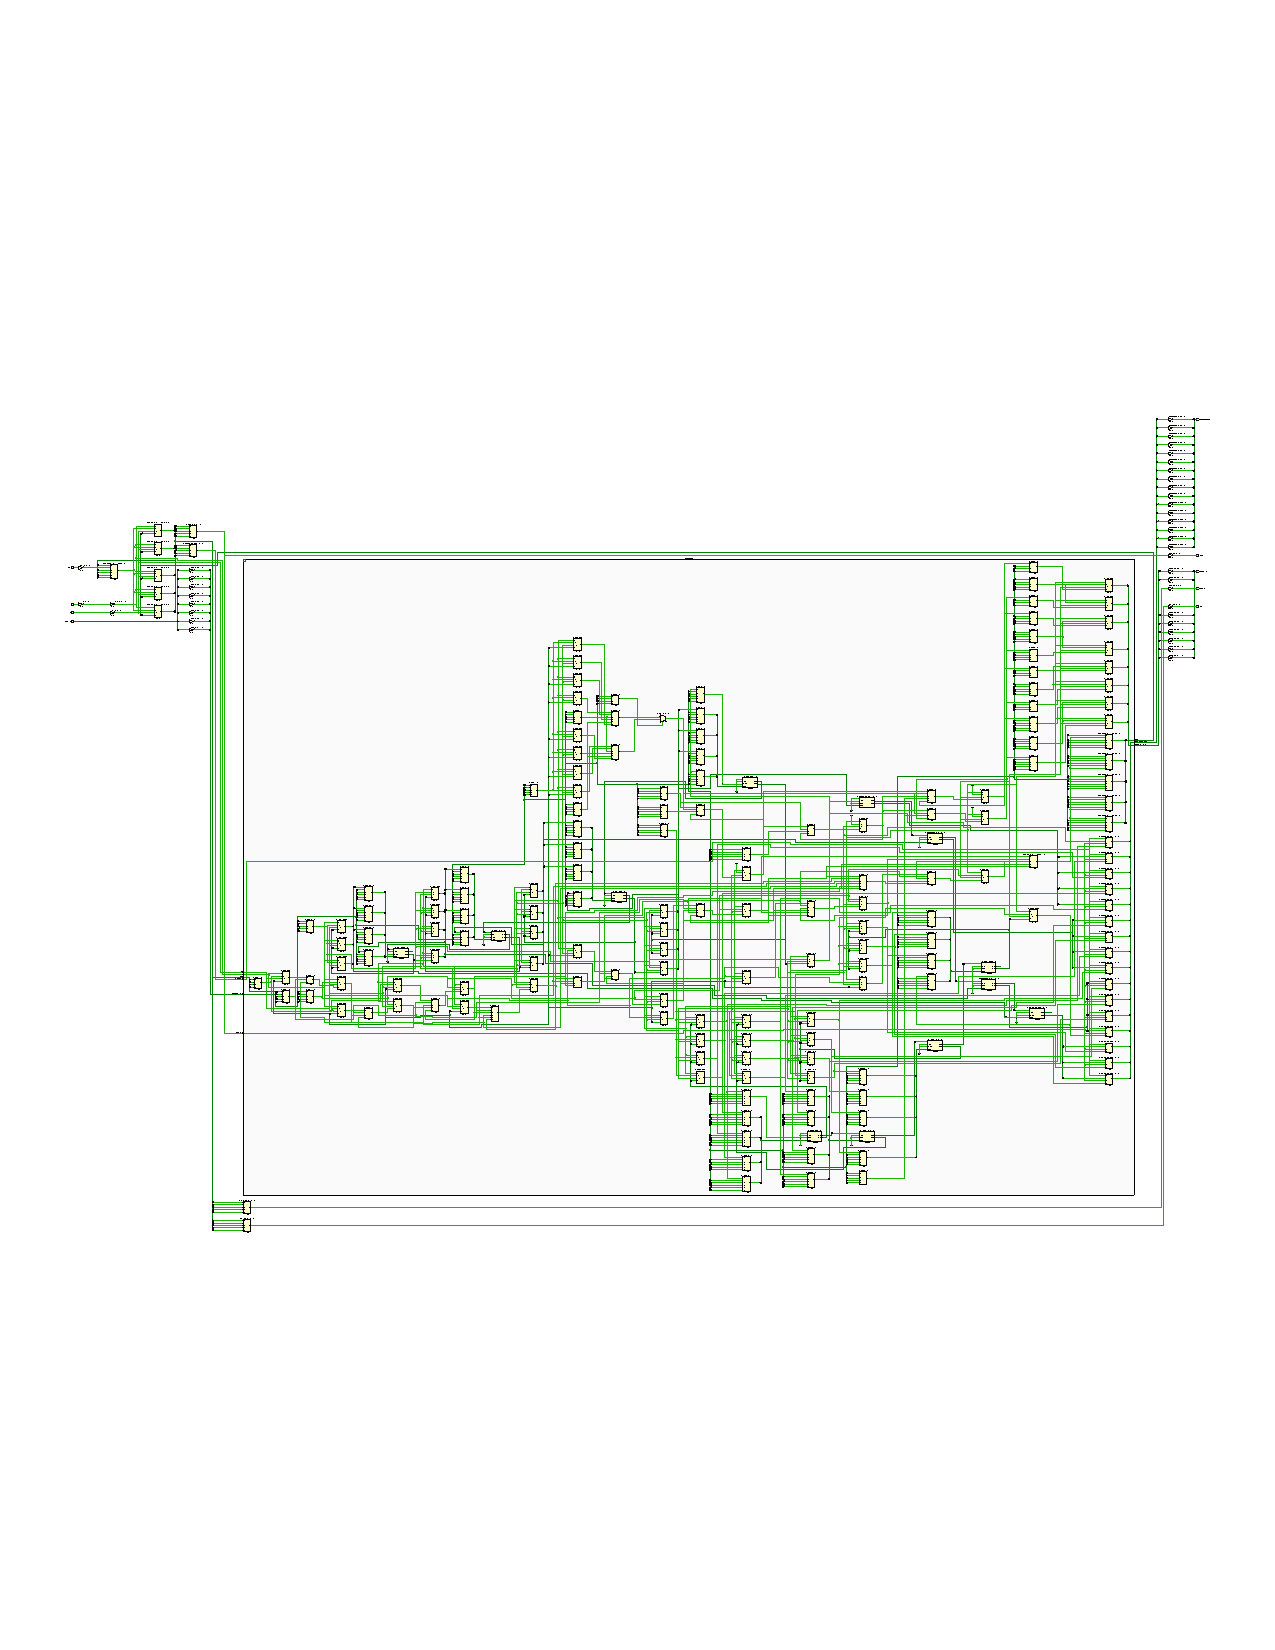
\includegraphics[width=1.1\textwidth]{PostSynthesis_Opened_Schematic.pdf}
				\caption{Circuto in post-sintesi completo}
				\label{fig:Schematic_PostSynthesis_Opened}
			\end{figure}
		%
		\subsection{Simulazioni}
			In questa sezione andremo a descrivere i casi di test fornitici e come questi ci 
			hanno permesso di comprendere meglio cosa non funzionasse nel nostro componente, 
			fino all'esecuzione corretta di tutti i test.
			%
			\subsubsection{Test bench : "tb\_seq\_min"}
				In questo test bench si vuole verificare che non avvenga alcuna computazione dei 
				valori, nel caso in cui all'indirizzo di memoria 0 sia contenuto il valore 0000, 
				indicante l'assenza di parole negli indirizzi successivi. 
				Questo è verificato inserendo dei valori nelle celle di memoria seguenti
				e controllando che agli indirizzi di scrittura le celle rimangano identificamente nulle.
				
				\textbf{Considerazione:} questo tb ci ha permesso di comprendere quale fosse il nostro problema 
				nella gestione del segnale di $o_{end}$, facendoci rendere conto di un errore  in fase di
				dichiarazione dei segnali.
				%
			\subsubsection{Test bench : "tb\_reset"}	
				In questo test bench si vuole verificare la corretta gestione di un segnale di reset,
				che viene impostato alto asincronamente rispetto all’usuale utilizzo del componente.
				
			\subsubsection{Test bench :  "tb\_re\_encode"}
				In questo test bench viene effettuato il controllo sulla correttezza della gestione 
				di segnali di tipo $i_{start}$, senza l’utilizzo del segnale di reset $i_{rst}$. 
				E’ perciò possibile comprendere se il componente descritto è in grado 
				di iniziare nuovamente un ciclo di traduzione senza essere esplicitamente 
				resettato allo stato $S0$.
			
			\subsubsection{Test bench : "tb\_doppio\_uguale"}
				In questo test bench viene effettuato il controllo sulla corretta lettura e scrittura 
				dei dati dalla memoria. Viene infatti controllato che i dati presenti all’inizio del test 
				siano gli stessi presenti dopo la prima esecuzione della routine che viene 
				doppiamente ripetuta: garantisce perciò che i dati presenti in memoria 
				vengano correttamente letti, ma non sovrascritti.
				
			\subsubsection{Test bench : "tb\_seq\_max "}
				In questo test bench viene effettuato il controllo sull’utilizzo del componente 
				con una sequenza avente la massima lunghezza possibile.
				
			\subsubsection{Test bench : "tb\_tre\_reset "}
				In questo test bench viene effettuato il controllo del funzionamento del 
				componente in caso di segnale di reset venga attivato più volte.
				
	%
%------------------------------------------------------------------------------------------------------------
%	SECTION 4 - CONCLUSIONS
%------------------------------------------------------------------------------------------------------------
	%
	\section{Conclusioni}
	
		Dai risultati sperimentali e dalla sintesi ottenuta riteniamo che l'architettura
		progettata del codificatore convoluzionale rispetti le specifiche
		richieste. I casi di test fornitici sono stati eseguiti correttamente e
		hanno contribuito al raffinamento del progetto fino al momento della consegna.
		\newline
		
		La descrizione hardware tramite linguaggio VHDL è completamente diversa dai 
		linguaggi di programmazione, perciò durante la definizione del progetto abbiamo 
		incontrato diversi problemi relativi ad alcune errate o mancanti considerazioni. 
		
		Grazie al lavoro svolto sul progetto abbiamo guadagnato la capacità di modificare 
		il livello di astrazione con cui pensare al progetto, dovendo passare da alto 
		a basso livello di astrazione, e viceversa, per capire come effettivamente 
		occorresse descrivere il componente. Questa è stata dunque una possibilità 
		per slegarci dal puro punto di vista del programmatore e dunque di poterci porre 
		delle domande sull’effettivo funzionamento dei componenti fisici dei quali 
		talvolta ignoriamo la complessità e l’utilizzo.
	
%
\end{document}